%------------------------------------------------------------------------
\begin{frame}
  \frametitle{}
  \begin{center}
    \textbf{\Large A pseudospectral method for pitch-angle scattering}
  \end{center}
\end{frame}
%------------------------------------------------------------------------

%------------------------------------------------------------------------
\begin{frame}
  \frametitle{Example from kinetic theory\\
    \csub{\small Legendre Pseudospectral method for pitch-angle scattering}}
  \begin{tcolorbox}
    \begin{equation*}
      \frac{\partial f}{\partial t} = \nu \frac{\partial}{\partial x}
      (1-x^2) \frac{\partial f}{\partial x} 
    \end{equation*}
  \end{tcolorbox}
  \begin{itemize}
  \item<1-> Time-evolution due to \hilite{pitch-angle scattering}
  \item<2-> Start with $f(t)$
  \item<3-> Evolve to $f(t+\Delta t)$
  \item<4-> Should conserve number
    \begin{equation}
      \frac{\partial }{\partial t} \int_{-1}^{1} dx \, f(x) = 0
    \end{equation}
    \item<5-> No conditions at $x=\pm 1$ except regularity
  \end{itemize}
\end{frame}
%------------------------------------------------------------------------
\begin{frame}
  \frametitle{Example from kinetic theory\\
    \csub{\small Legendre Pseudospectral method for pitch-angle scattering}}
  \begin{tcolorbox}
    \begin{equation*}
      \frac{\partial f}{\partial t} = \nu \frac{\partial}{\partial x}
      (1-x^2) \frac{\partial f}{\partial x} 
    \end{equation*}
  \end{tcolorbox}
  \begin{itemize}
  \item<1->We can move between node and spectral bases  
    \begin{equation*}
      f(x_i) = \sum_n c_n P_n(x_i) \longrightarrow f_i = A_{in} c_n \quad \text{where} \quad A_{in} = P_n(x_i) 
    \end{equation*}
    \item<2->The evolution equation at node $i$ becomes  
    \begin{align*}
      \frac{\partial f_i}{\partial t} = & -\nu \sum_n n(n+1) c_n P_n(x_i)
      = -\nu L_{in} c_n \\
      & \text{where} \quad L_{in} = n(n+1)P_n(x_i)  
    \end{align*}
    \end{itemize}
 \end{frame}
%------------------------------------------------------------------------
\begin{frame}
  \frametitle{Legendre Pseudospectral method for pitch-angle scattering\\
    \csub{\small Timestep is a matrix-vector multiply}}
  \begin{tcolorbox}
    \begin{equation*}
      \frac{\partial f}{\partial t} = \nu \frac{\partial}{\partial x}
      (1-x^2) \frac{\partial f}{\partial x} 
    \end{equation*}
  \end{tcolorbox}
  \begin{itemize}
    \item <1->The evolution equation at node $i$ is 
    \begin{align*}
  \frac{\partial f_i}{\partial t} = -\nu C_{ik} f_k \qquad C_{ik} = &~L_{in} (A^{-1})_{nk} \\
      L_{in} = &~n(n+1)P_n(x_i) \\
      A_{in} = &~P_n(x_i)
    \end{align*}
    \item<2-> Implicit time advance, with $\bar{f} = f(t+\Delta t)$
    \begin{equation*}
\frac{\bar{f}_i-f_i}{\Delta t} = -\nu C_{ik} \bar{f}_k \quad \longrightarrow\quad
      \left(\delta_{ik} + \nu \Delta t C_{ik} \right) \bar{f}_k = f_i
    \end{equation*}
  \end{itemize}
\end{frame}
%------------------------------------------------------------------------
%------------------------------------------------------------------------
\begin{frame}
  \frametitle{Legendre Pseudospectral method for pitch-angle scattering\\
    \csub{\small Timestep is a matrix-vector multiply}}
  \begin{tcolorbox}
    \begin{equation*}
      \frac{\partial f}{\partial t} = \nu \frac{\partial}{\partial x}
      (1-x^2) \frac{\partial f}{\partial x} 
    \end{equation*}
  \end{tcolorbox}
  \begin{itemize}
  \item <1->Spectrally-accurate discrete approximation
    \begin{equation*}
      \bar{f}_k = M_{ik} f_i
    \end{equation*}
  \item<2->Conserves number to machine precision
  \item<3->Regularity at $x=\pm 1$ without accuracy loss or instability
  \item<4->Matrix-vector multiply (DGEMV) well-suited for multicore or accelerator optimization
  \end{itemize}
\end{frame}
%------------------------------------------------------------------------
%------------------------------------------------------------------------
\begin{frame}
  \frametitle{Legendre Pseudospectral method for pitch-angle scattering\\
    \csub{\small Density exactly conserved ; smooth solutions a boundaries}}
  \begin{center}
    \vskip -1cm
      \only<1>{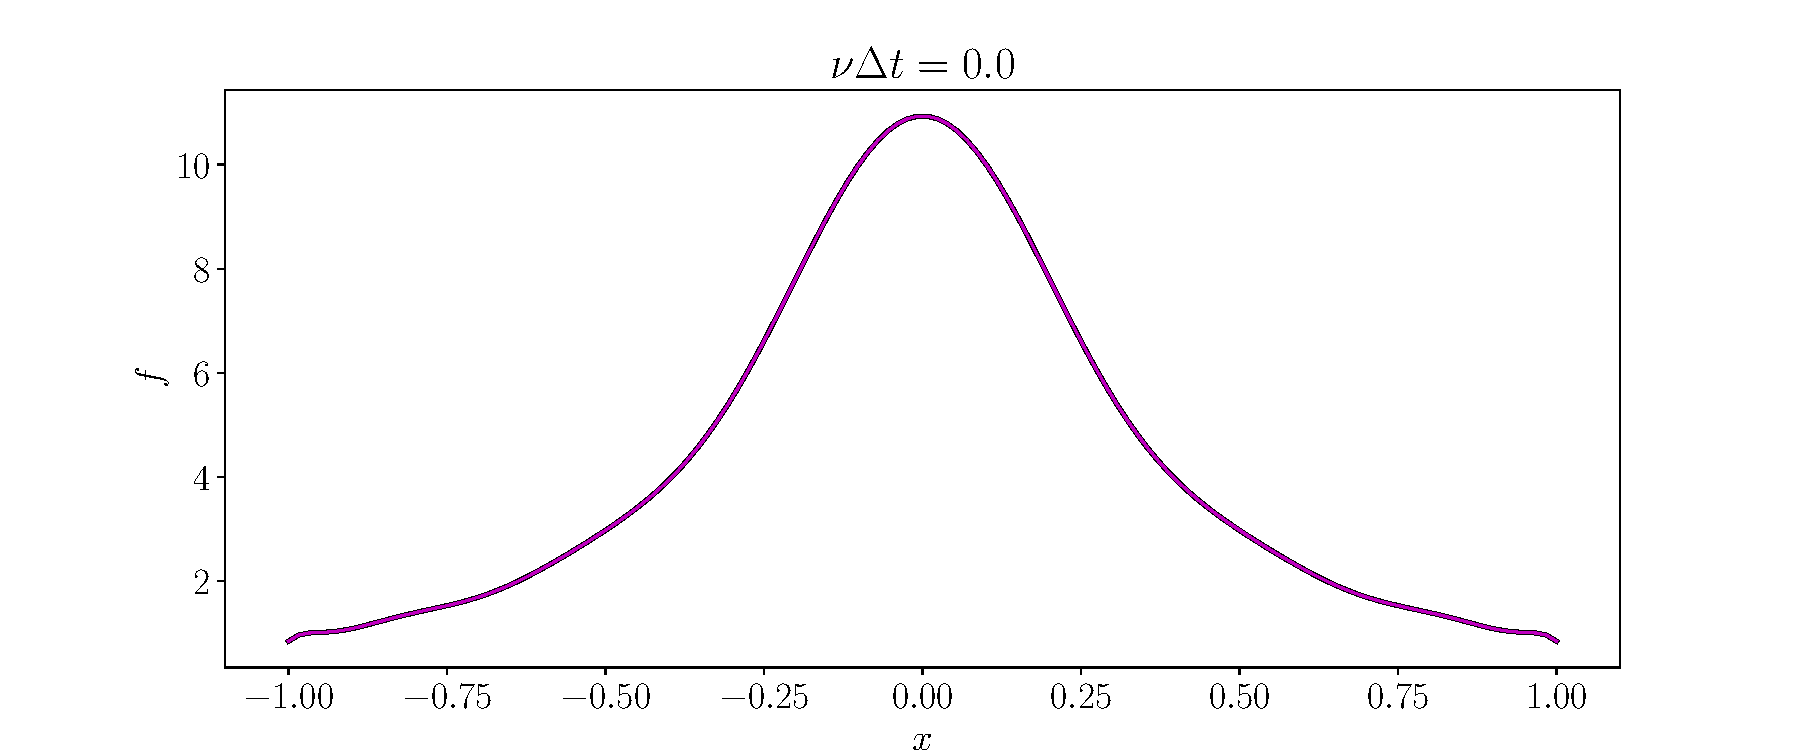
\includegraphics[width=16cm]{pitch0.pdf}}%
      \only<2>{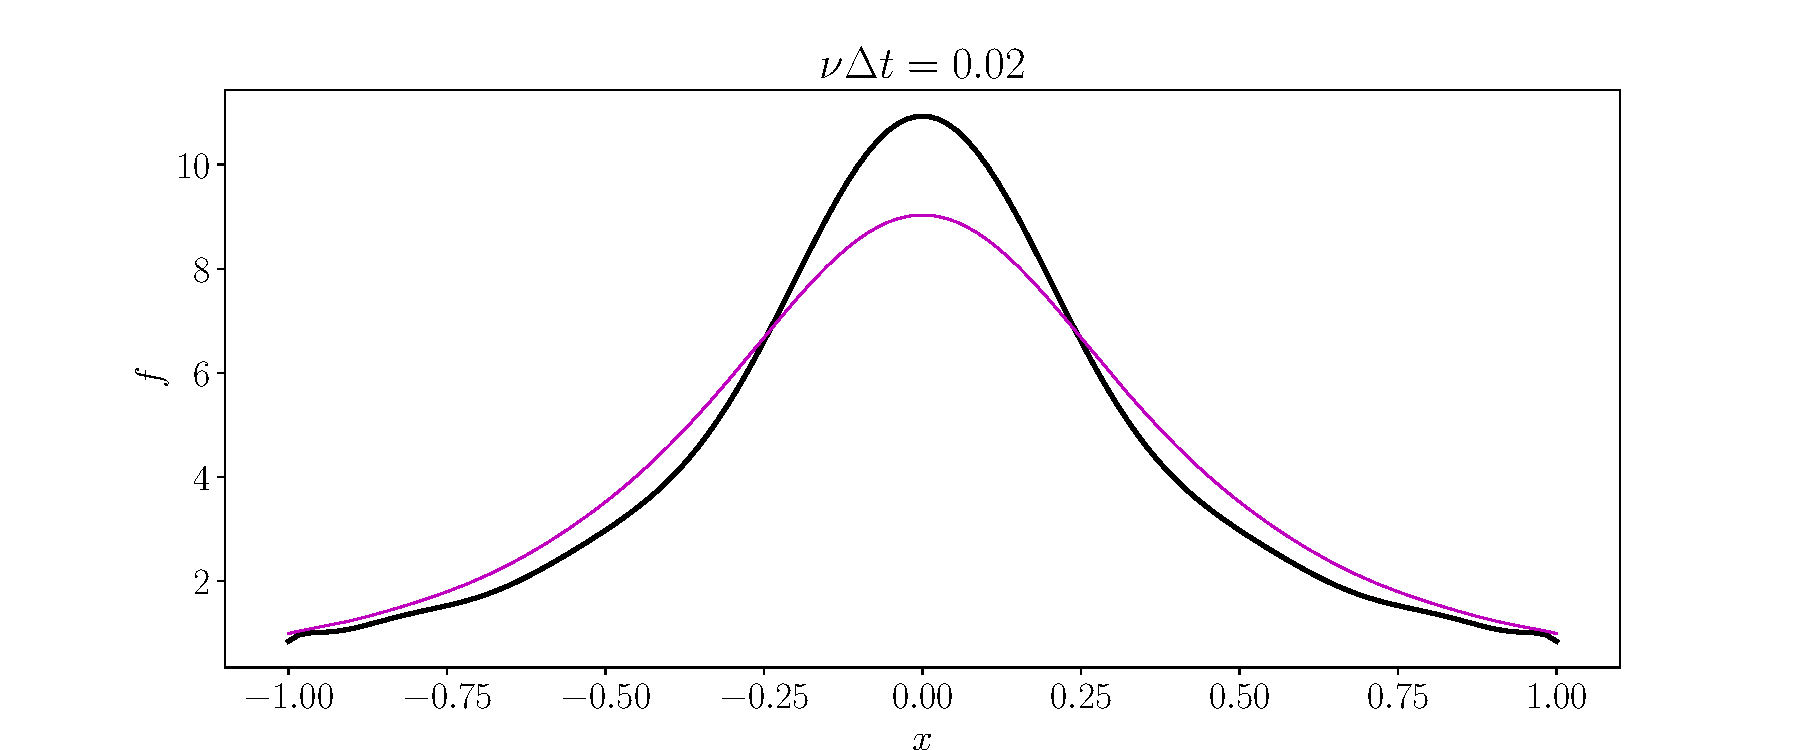
\includegraphics[width=16cm]{pitch1.pdf}}%
      \only<3>{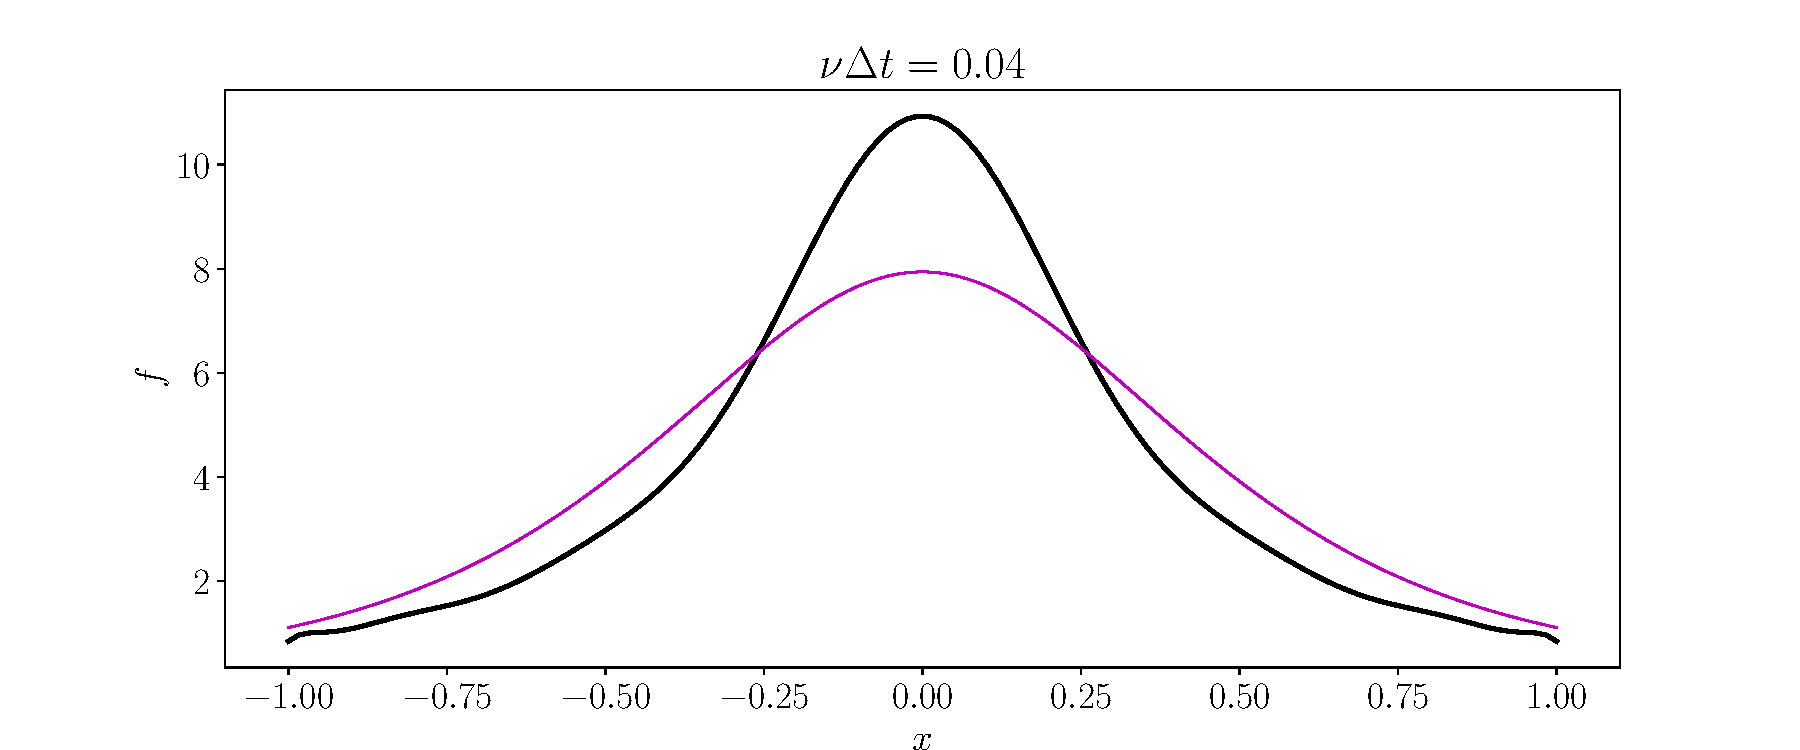
\includegraphics[width=16cm]{pitch2.pdf}}%
      \only<4>{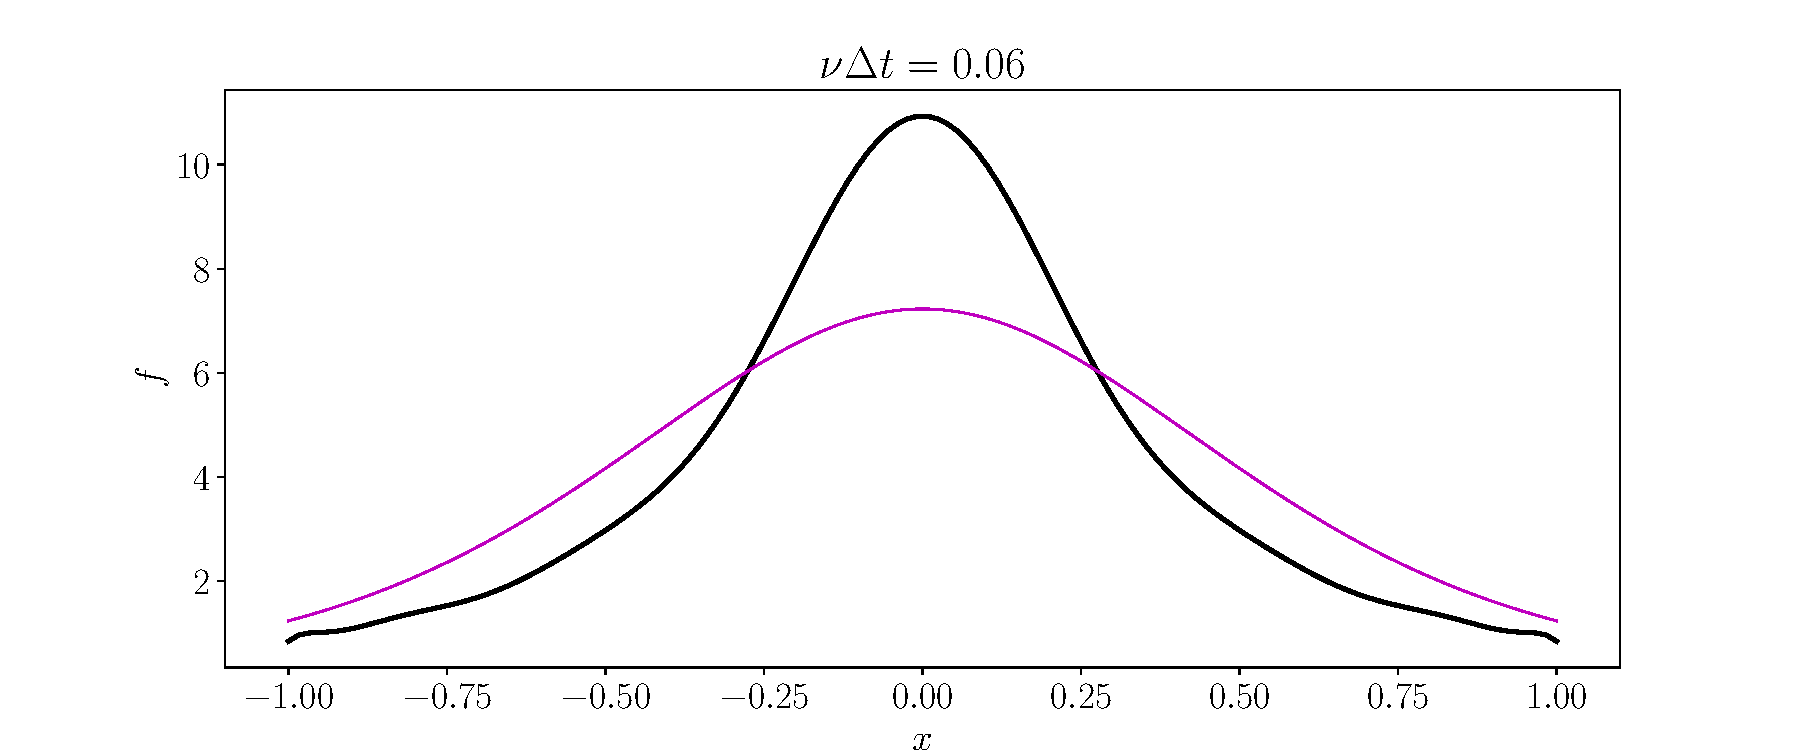
\includegraphics[width=16cm]{pitch3.pdf}}%
      \only<5>{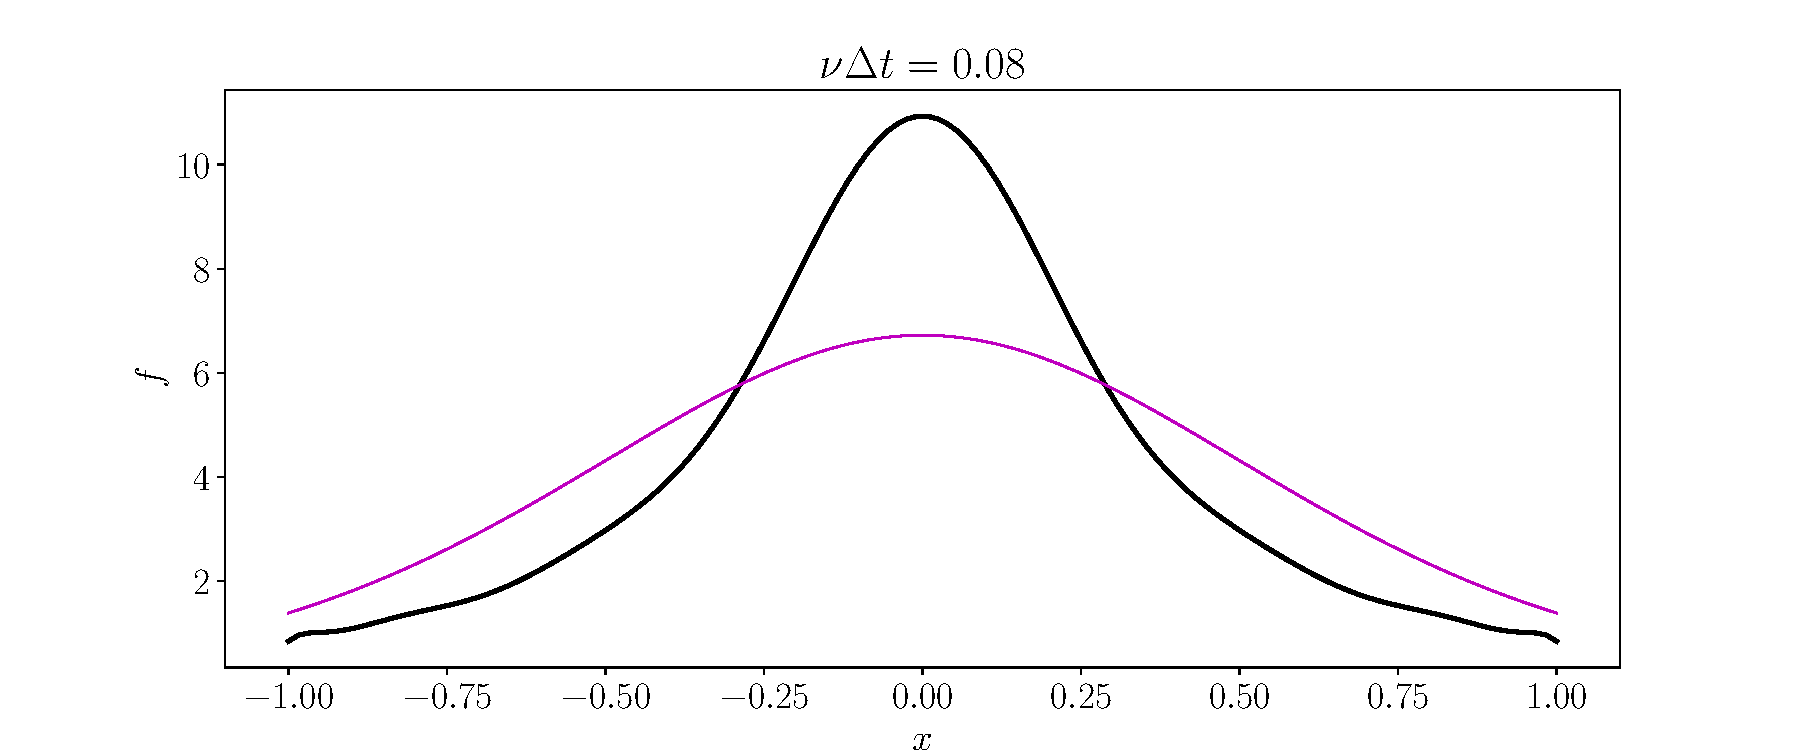
\includegraphics[width=16cm]{pitch4.pdf}}%
      \only<6>{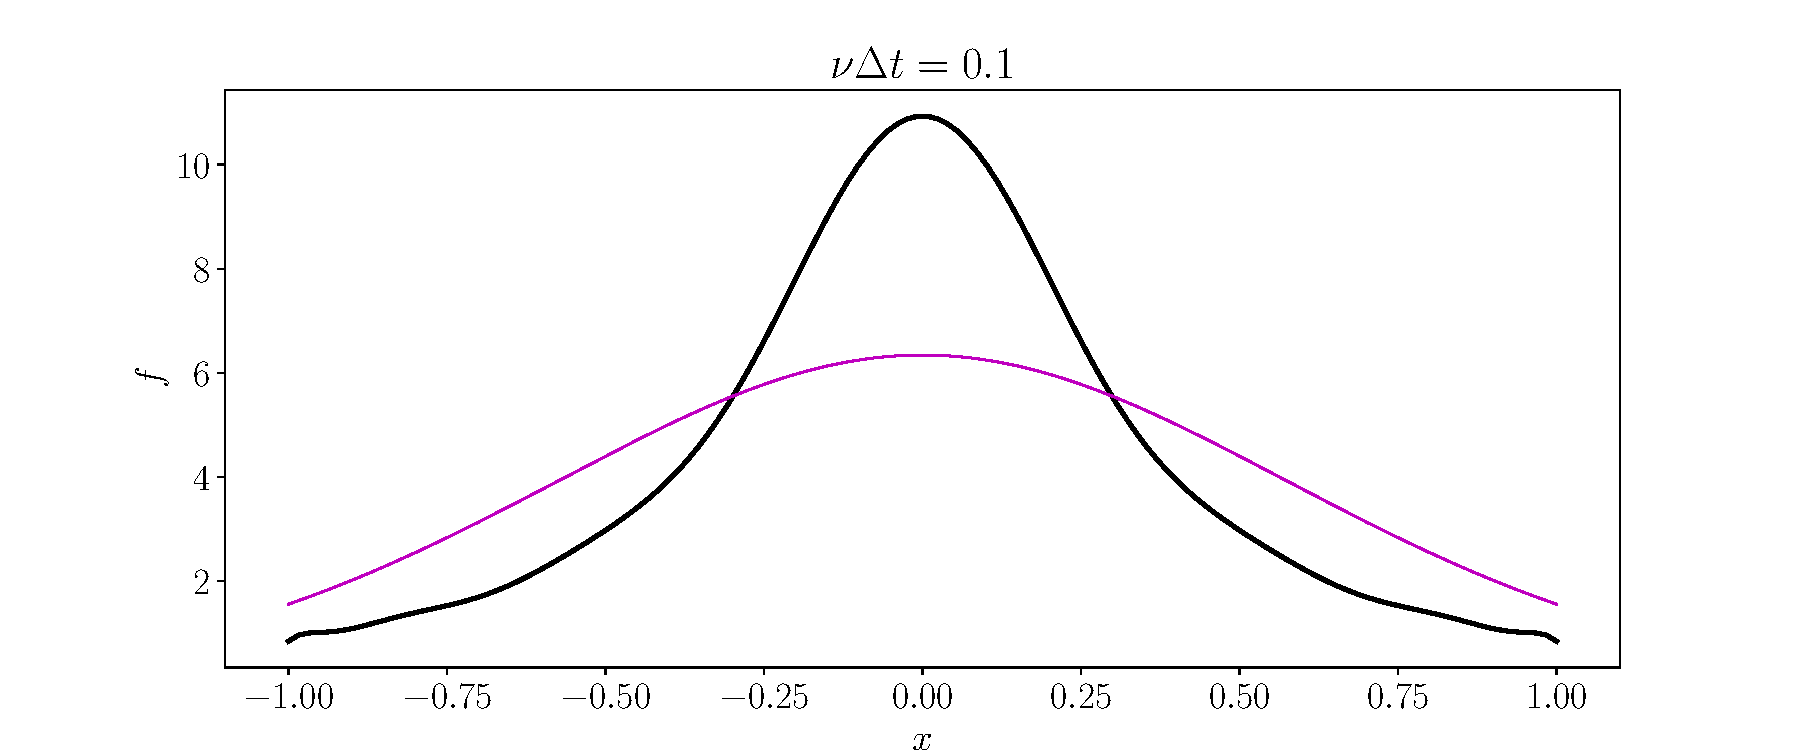
\includegraphics[width=16cm]{pitch5.pdf}}%
      \only<7>{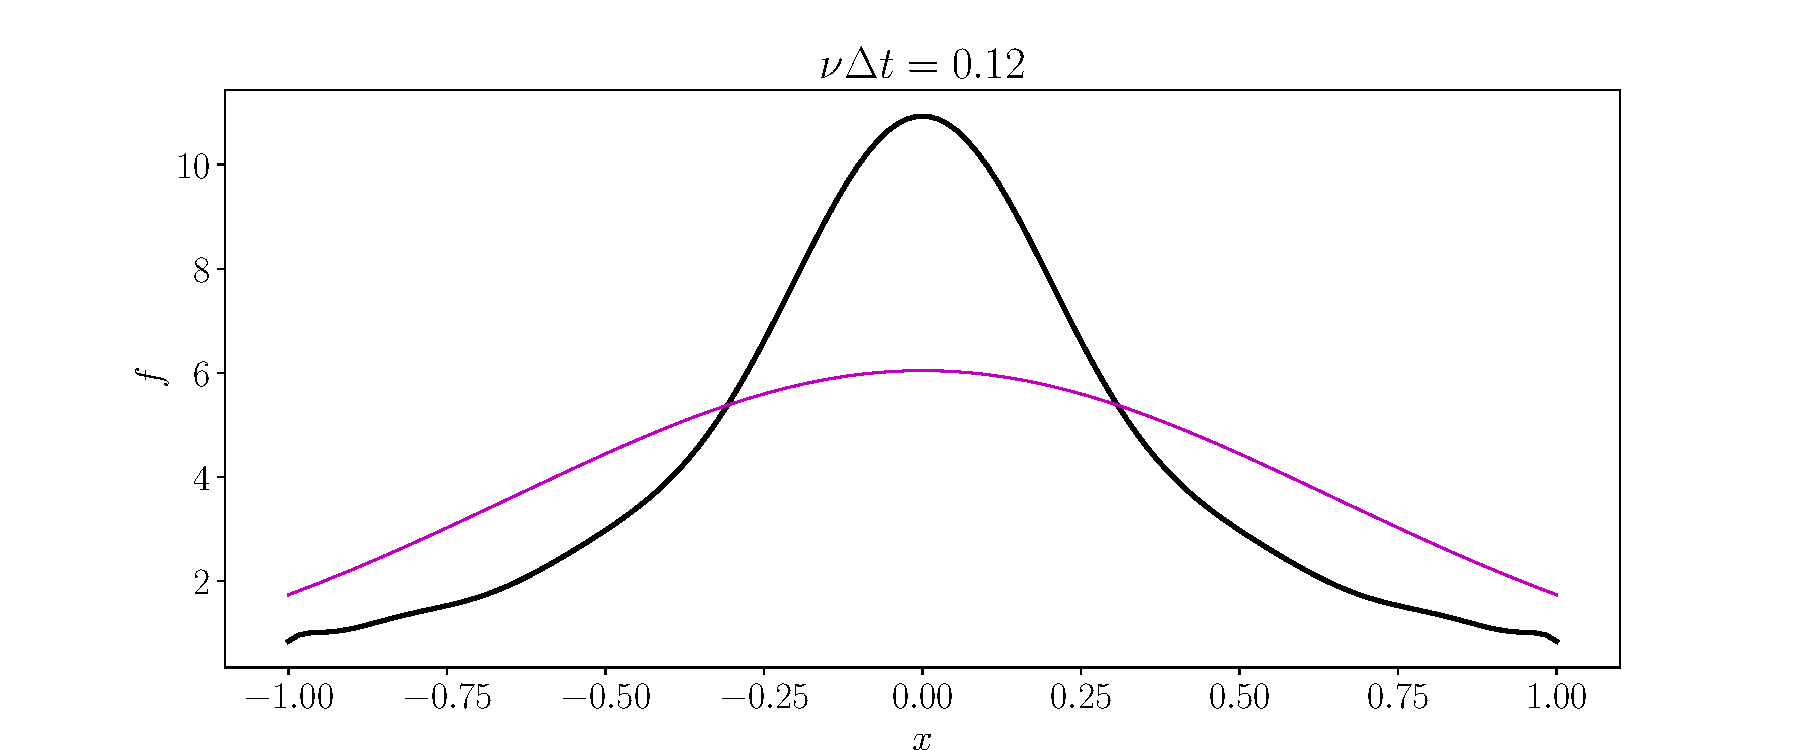
\includegraphics[width=16cm]{pitch6.pdf}}%
      \only<8>{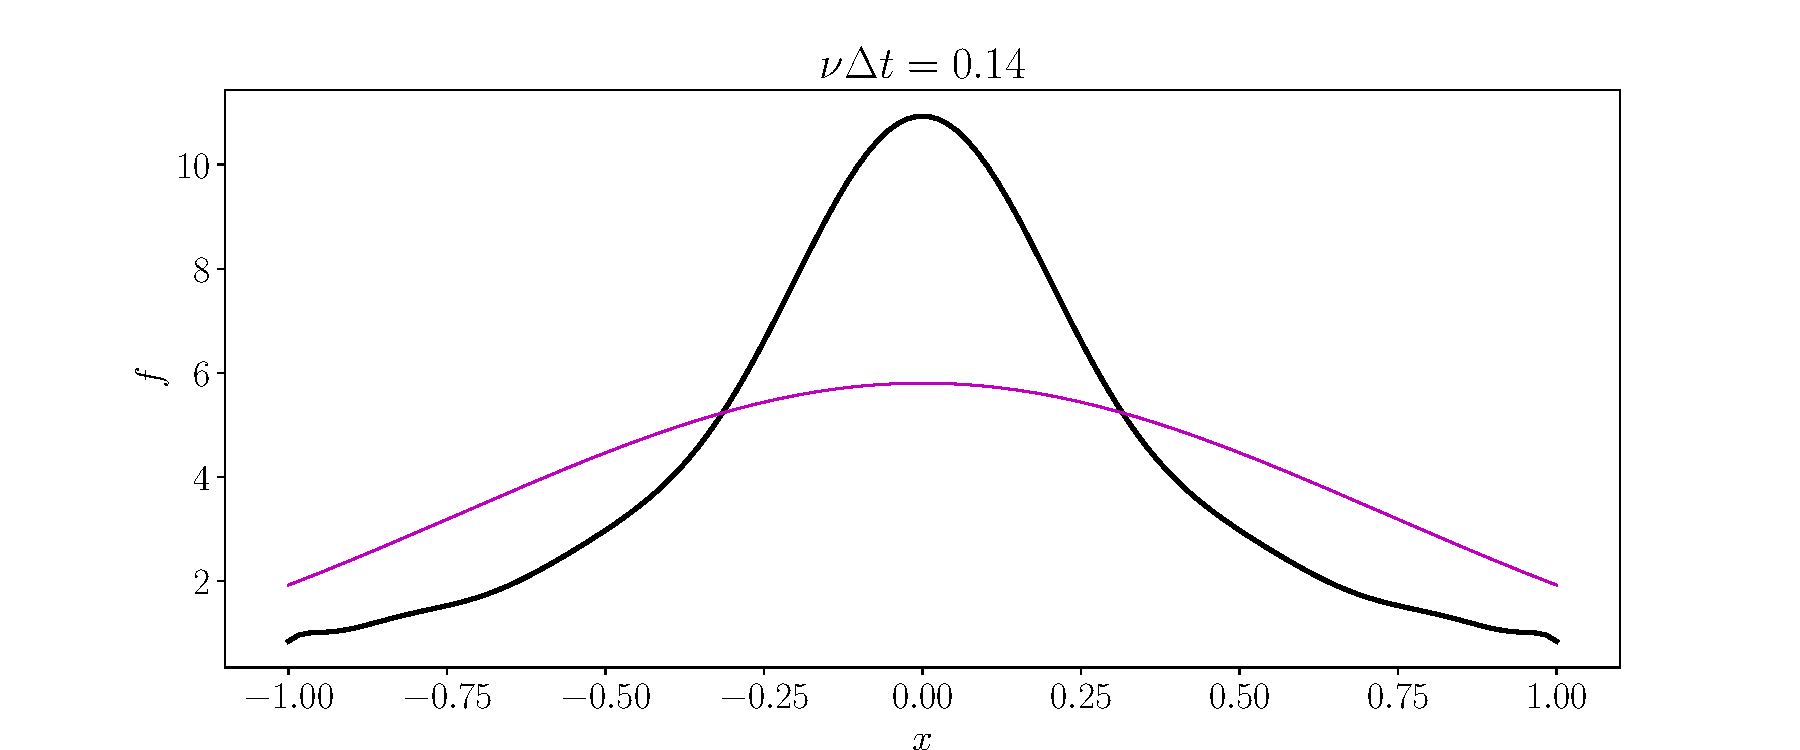
\includegraphics[width=16cm]{pitch7.pdf}}%
      \only<9>{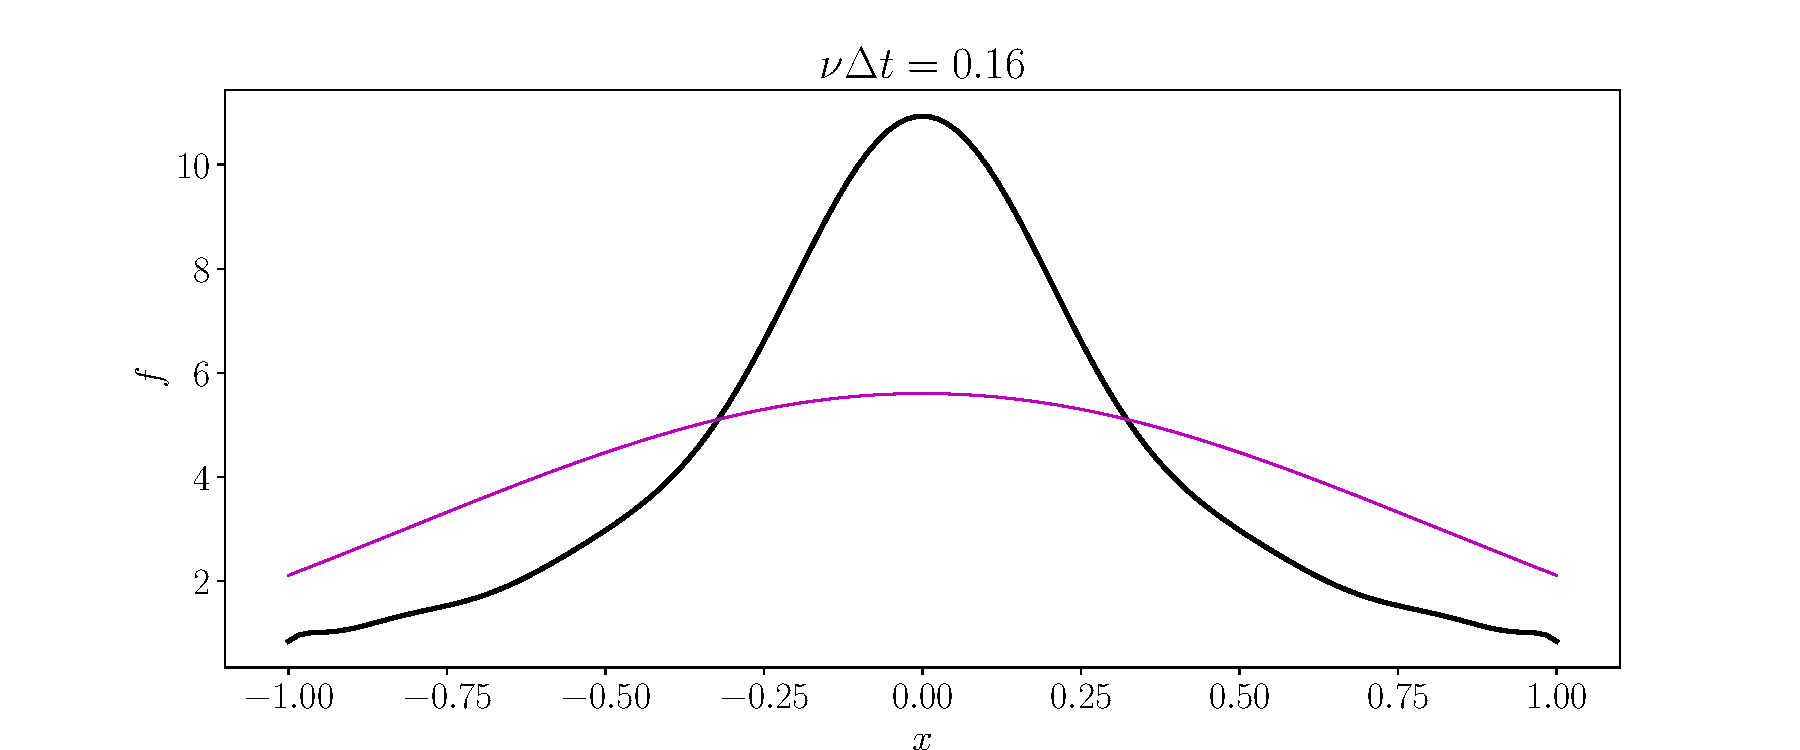
\includegraphics[width=16cm]{pitch8.pdf}}%
      \only<10>{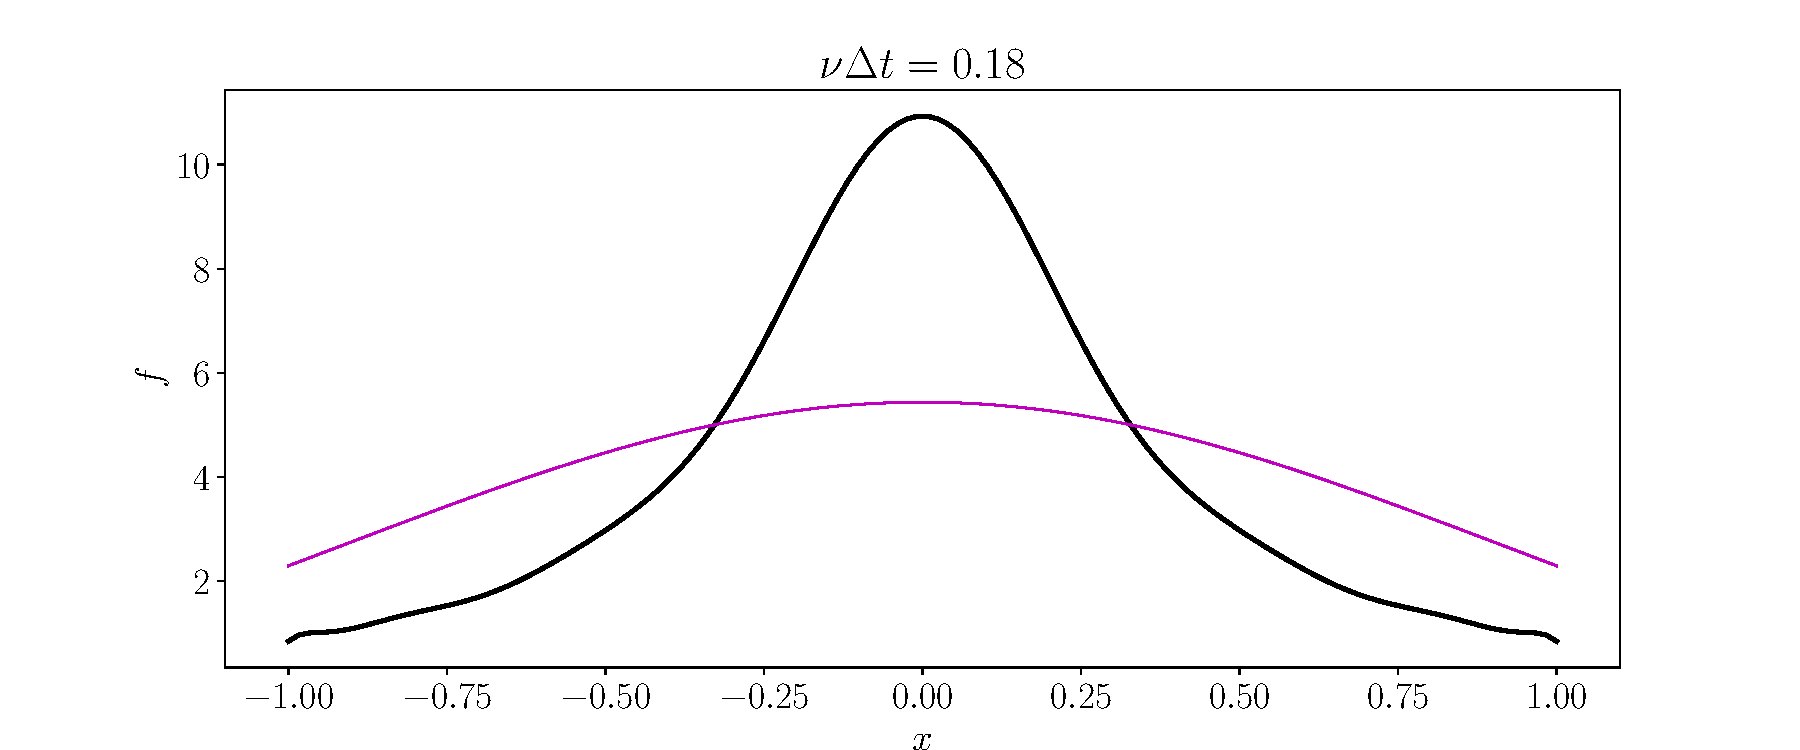
\includegraphics[width=16cm]{pitch9.pdf}}%
      \only<11>{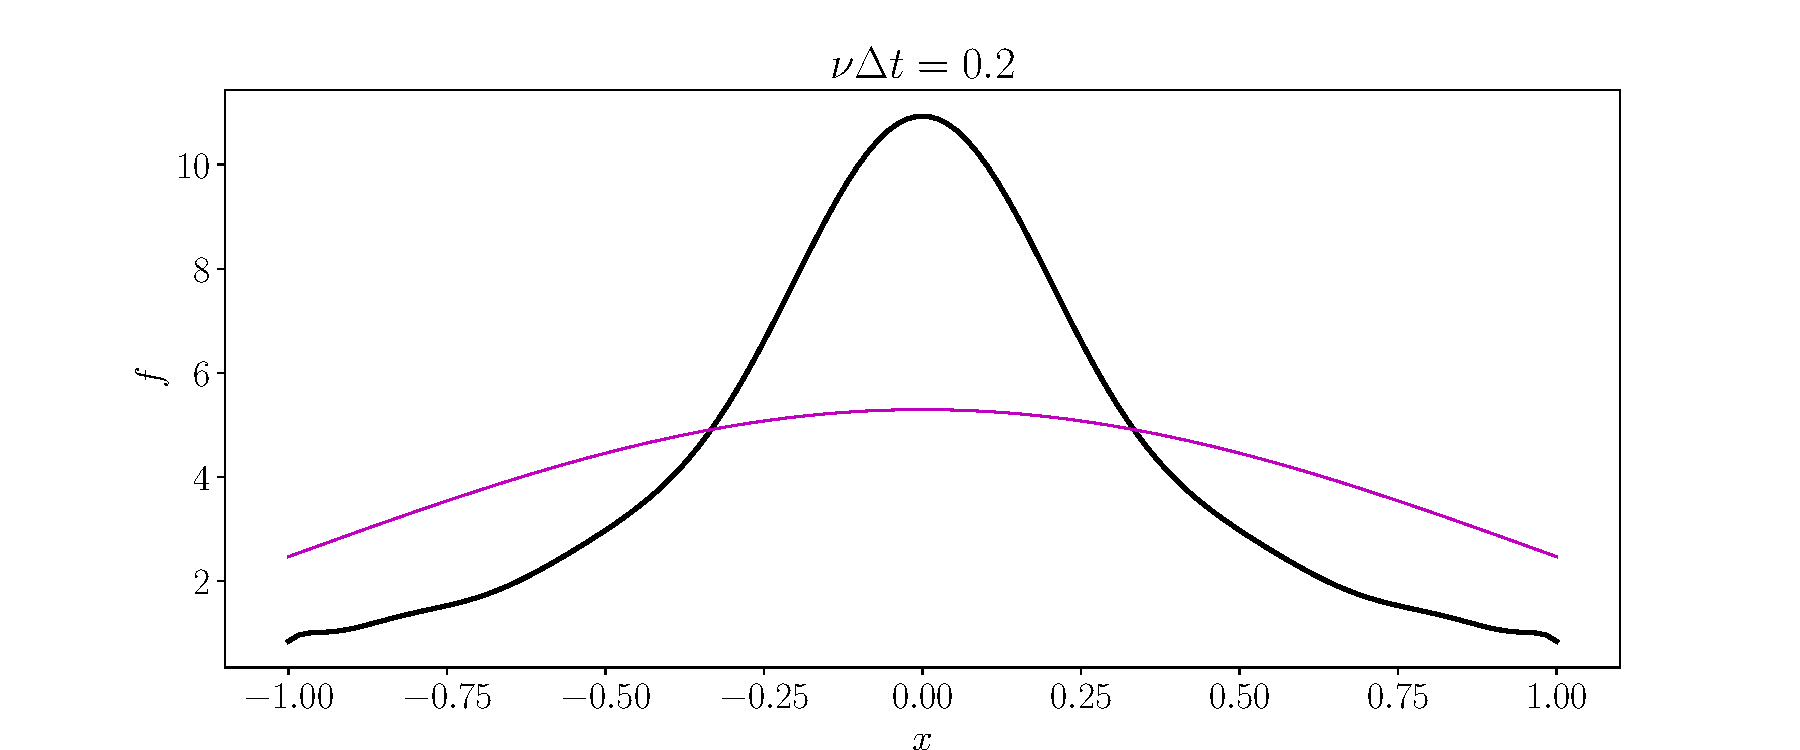
\includegraphics[width=16cm]{pitch10.pdf}}%
      \only<12>{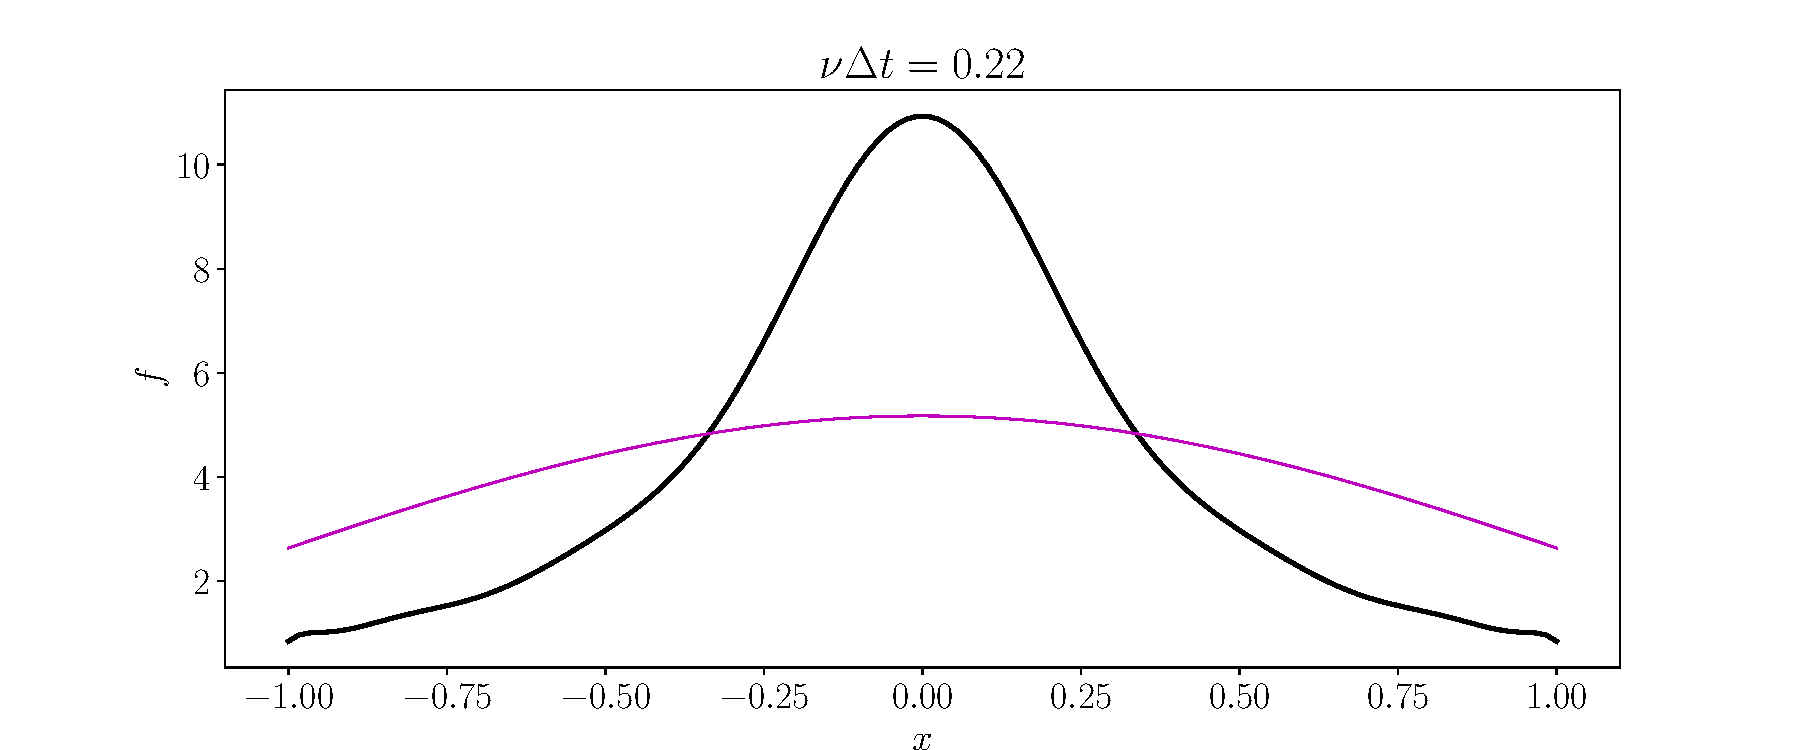
\includegraphics[width=16cm]{pitch11.pdf}}%
      \only<13>{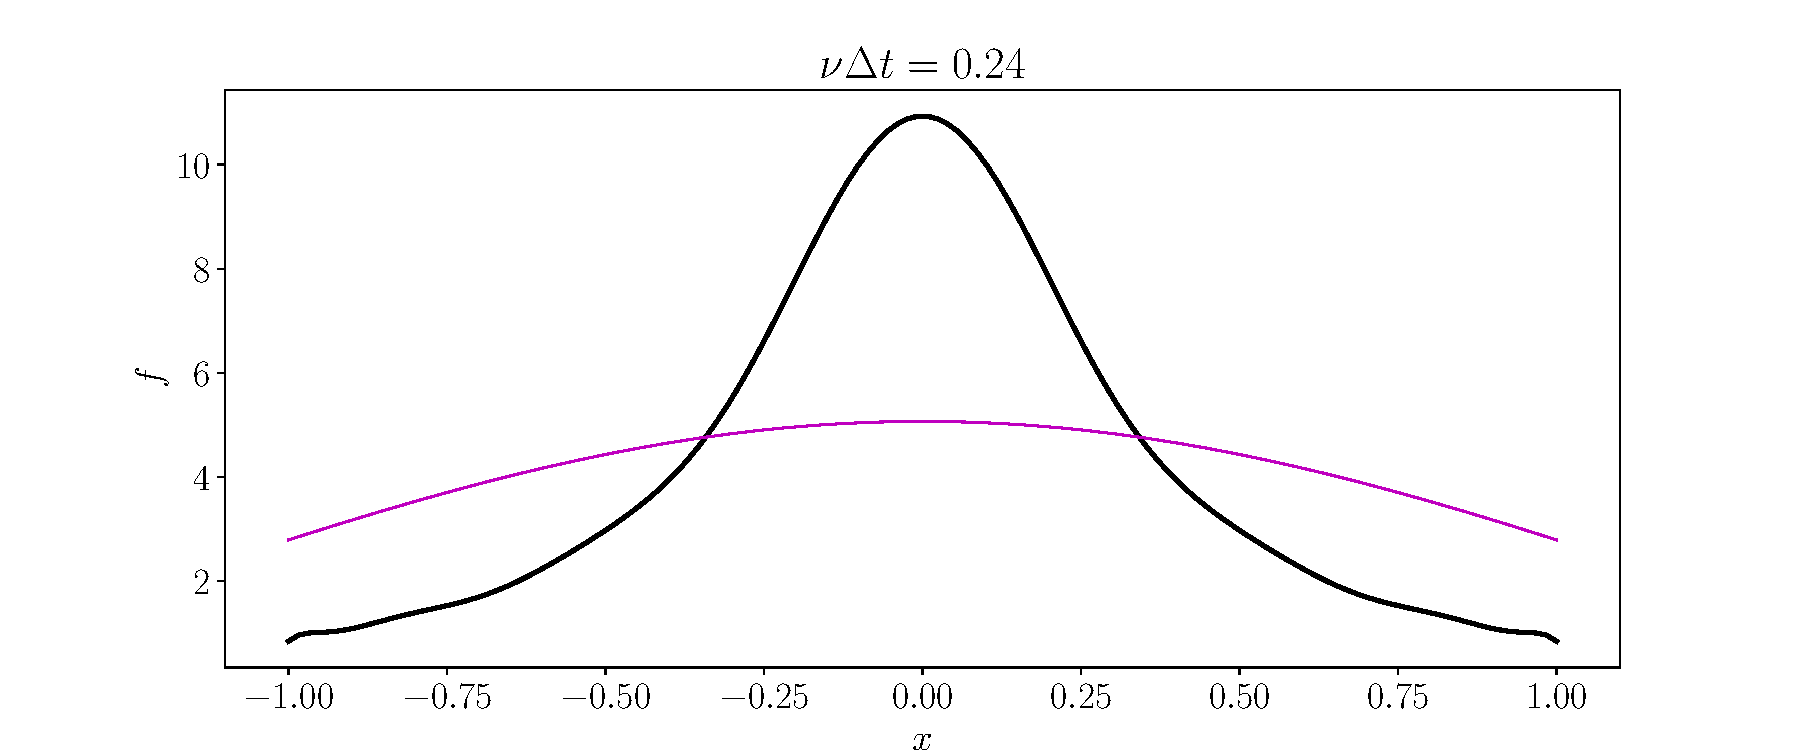
\includegraphics[width=16cm]{pitch12.pdf}}
  \end{center}
\end{frame}
%------------------------------------------------------------------------
